\documentclass[12pt]{beamer}
\usepackage[utf8]{inputenc}
\usepackage[spanish]{babel}
%\usepackage{graphicx}
%\usepackage[pdftex]{hyperref}
\usepackage{listings}
\usepackage{eurofont}
\usepackage{lmodern}
\usepackage{transparent}

%\usetheme{Warsaw}
%\mode<presentation>
%{ \usetheme{boxes} }


\newcommand{\mysection}[1]{\begin{frame}{}\begin{center}\Huge #1\end{center}\end{frame}}

% Comment the next line to create a printable version
\beamerdefaultoverlayspecification{<+->}
\setbeamercovered{transparent}
\usepackage{keynote-gradient}

\title{Programación mediante tarjetas gráficas}
\subtitle{Mejora de una aplicación distribuida}
\author{Samuel Rodríguez Sevilla\\Tutor: José María Sierra Cámara}


\begin{document}


\frame{\titlepage}

%\begin{frame}
%	\begin{center}
%		\Huge iCrack
%	\end{center}
%\end{frame}


\begin{frame}{Contenidos}
	\tableofcontents[pausesections]
\end{frame}

\section{Introducción}
\mysection{Introducción}
\begin{frame}{Introducción}
	\begin{itemize}
		\item La seguridad es muy importante actualmente
		\item Hay muchos factores que afectan a la seguridad
		\begin{itemize}
			\item Fallos de programación de las aplicaciones
			\item Mala configuración de los sistemas
			\item Factores humanos
		\end{itemize}
	\end{itemize}
\end{frame}

\begin{frame}{Introducción}
	\begin{center}
		El factor humano es probablemente el que más afecta a la seguridad ya que no hay una verdadera concienciación sobre los peligros que entraña revelar claves.
	\end{center}
\end{frame}

\begin{frame}{Introducción}
	Por esto es importente
	\pause
	\begin{itemize}
		\item Disponer de buenas políticas para las contraseñas
		\item Utilizar herramientas para evaluar la calidad de los algoritmos utilizados
	\end{itemize}
\end{frame}

\subsection{Objetivos}
\begin{frame}{Objetivos}
	\begin{center}
		Obtener una herramienta capaz de evaluar algoritmos de seguridad y contraseñas haciendo uso de tarjetas gráficas.
	\end{center}
\end{frame}

\begin{frame}{Objetivos}
	\begin{itemize}
		\item Sencilla de utilizar
		\item Ampliable con nuevos algoritmos
		\item Distribuida
		\item Libre
	\end{itemize}
\end{frame}

\subsection{Uso de tarjetas gráficas}
\begin{frame}{Uso de tarjetas gráficas}
	\begin{center}
%		Su velocidad ha crecido mucho~\cite{nvidia:cuda_c_programming_guide} y han añadido nuevas características que las hacen muy atractivas para todo tipo de tareas.
		Su velocidad ha crecido mucho y han añadido nuevas características que las hacen muy atractivas para todo tipo de tareas.
	\end{center}
\end{frame}


\lstset{emph={int,float,void}, emphstyle=\color{blue},
emph={[2]__global__,__device__,__kernel__,threadIdx},emphstyle={[2]\color{green}}}
\defverbatim[colored]\testcode{%
\begin{lstlisting}[frame=single%,%
%	backgroundcolor=\transparent{0.2}%
]
__global__ void vector_add(
  float *v1, float *v2, float *r)
{
  int p = threadIdx.x;
  r[p] = v1[p] + v2[p];
}
\end{lstlisting}}
\begin{frame}{Uso de tarjetas gráficas}
	Entre sus principales características destacan:
	\pause

	\begin{itemize}
		\item Una gran velocidad realizando operaciones aritméticas
		\only<2>{
			\begin{figure}
				\centering
				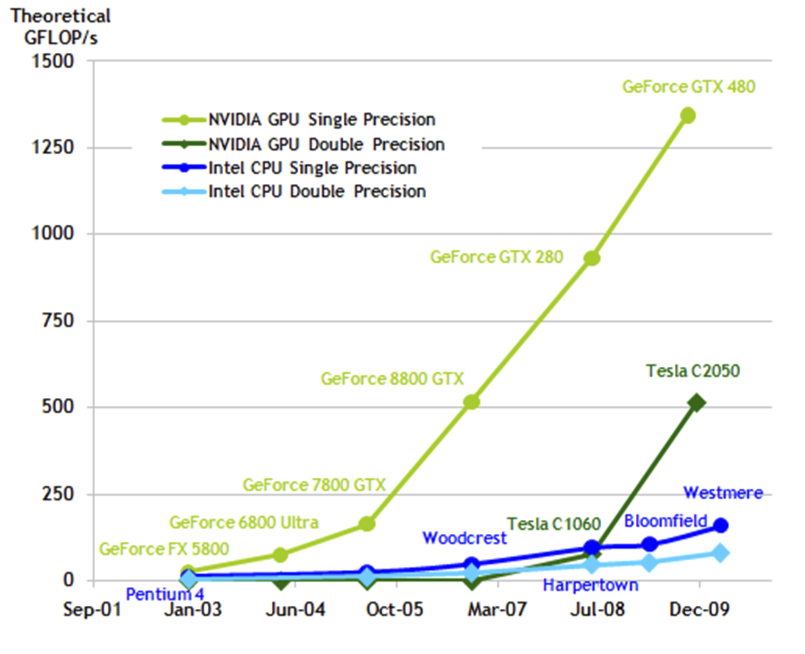
\includegraphics[width=0.5\textwidth]{images/evolucion-gpu.png}
%				\caption{Incremento de los FLOPS en CPU y GPU (fuente~\cite{nvidia:cuda_c_programming_guide})}
				\caption{Incremento de los FLOPS en CPU y GPU (fuente NVIDIA)}
			\end{figure}
		}

		\item Gran capacidad para el paralelismo
			\only<3>{
				\begin{figure}
					\centering
					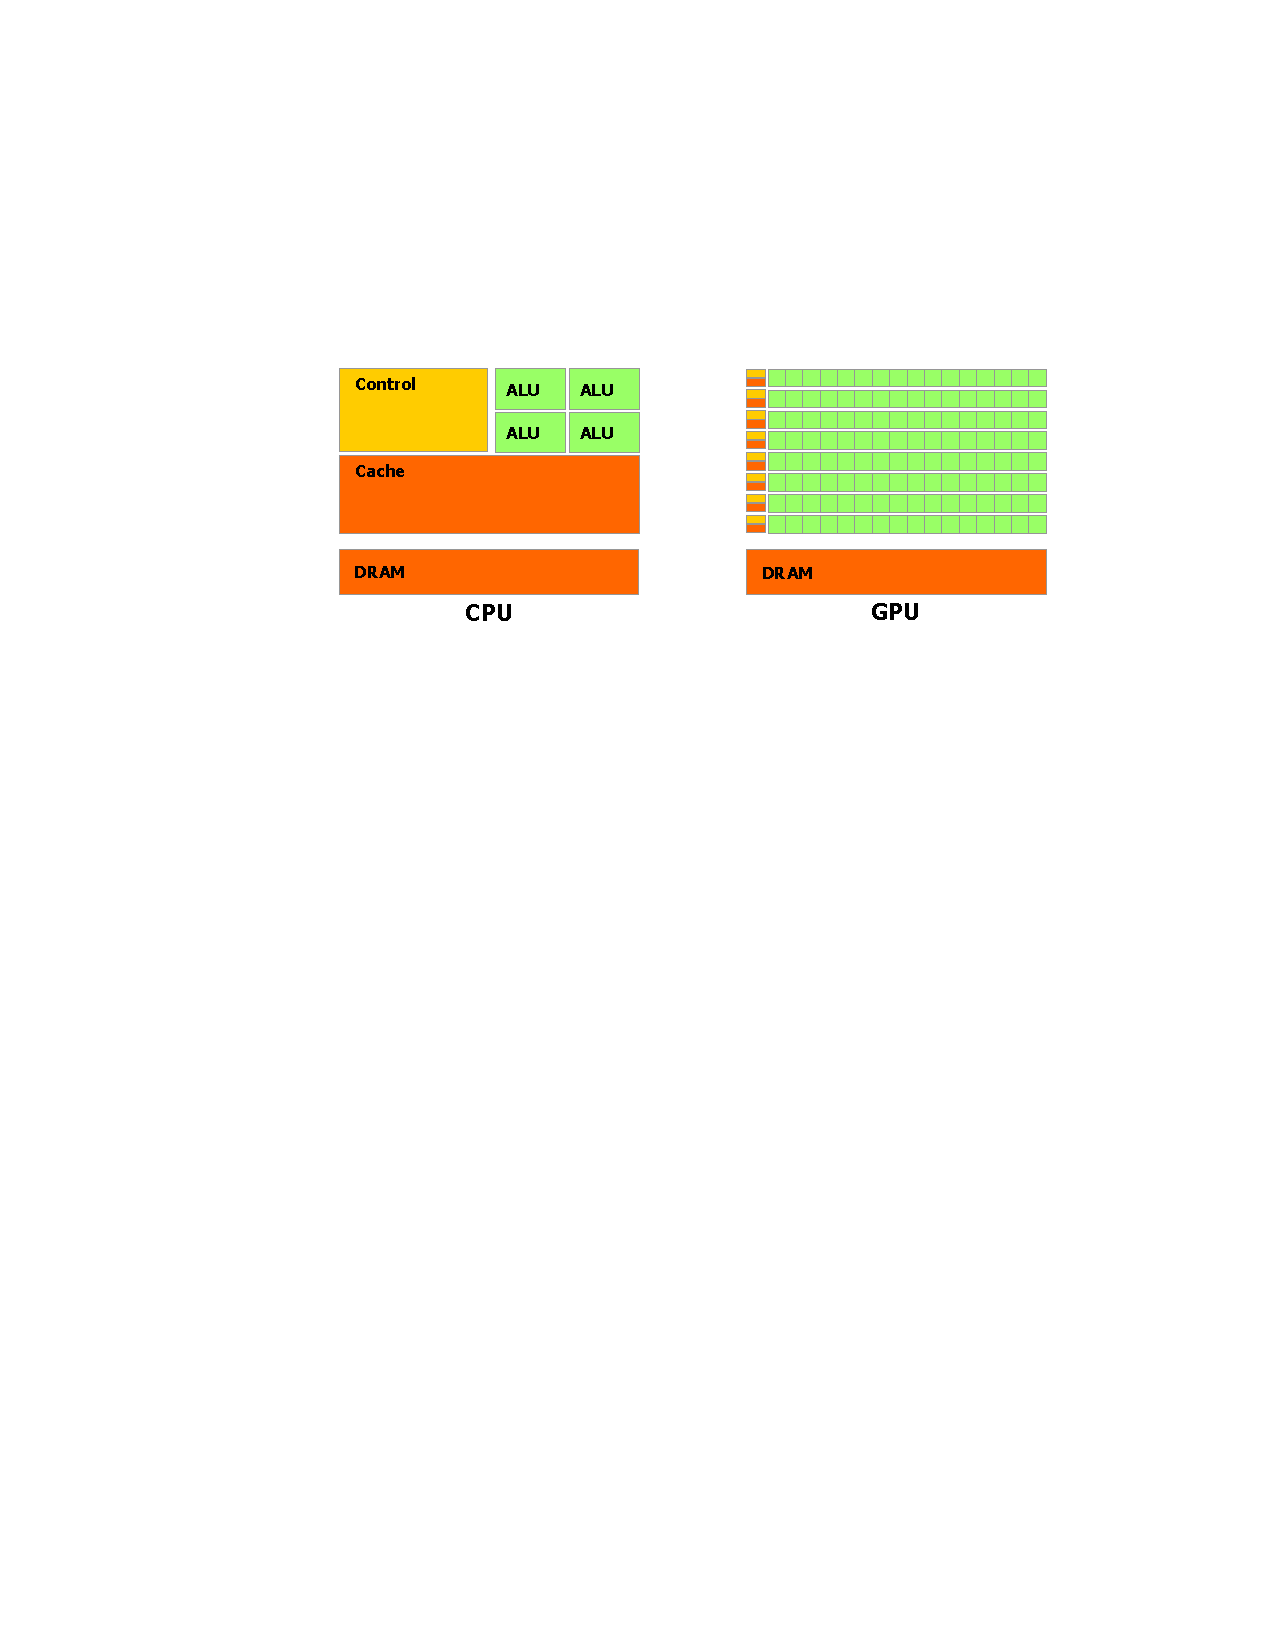
\includegraphics[width=0.7\textwidth]{images/cpuvsgpu.pdf}
%					\caption{Comparación interna CPU y GPU (fuente~\cite{nvidia:cuda_c_programming_guide})}
					\caption{Comparación interna CPU y GPU (fuente NVIDIA)}
				\end{figure}
			}

		\item Son fáciles de programar
			\only<4>{
				\testcode
			}
	\end{itemize}
\end{frame}

\section{DHC}
\mysection{DHC}
\begin{frame}{DHC}
	Se tomó como base de las modificaciones por varios motivos:
	\pause
	\begin{itemize}
		\item Es software libre
		\item Cumplía casi todos los requisitos
		\item Es la única herramienta gratuita de este tipo
	\end{itemize}
\end{frame}

\begin{frame}{DHC}
	Hay dos partes fundamentales:
	\pause
	\begin{itemize}
		\item El \color{green}Agente \color{white}que es la parte encargada del trabajo duro
		\item El \color{green}Controlador \color{white}que gestiona las tareas y el resparto de las mismas
	\end{itemize}
\end{frame}
\begin{frame}{DHC}
	\begin{center}
		Pero a pesar de todo, también tiene algunas carencias...
	\end{center}
\end{frame}


\section{Mejoras introducidas}

\mysection{Mejoras introducidas}

\subsection{SHA-256}
\begin{frame}
	Primera funcionalidad añadida. Nos permite evaluar:
	\pause
	\begin{itemize}
		\item La facilidad para ampliar DHC
		\item Comprender mejor la programación con tarjetas gráficas
	\end{itemize}
\end{frame}

\subsection{Mejora de la escalabilidad}
\begin{frame}{Mejora de la escalabilidad}
	DHC pierde mucha velocidad debido a:
	\pause
	\begin{itemize}
		\item Las latencias de red
		\item Gran cantidad de consultas desde los agentes
		\item Demasiados accesos a base de datos
	\end{itemize}
	% Esto se constata cuando se tiene una instalación...
\end{frame}

\begin{frame}{Mejora de la escalabilidad}
	Para solucionarlo se ha recurrido a espaciar las peticiones según:
	\pause
	\begin{itemize}
		\item Los tiempos de respuesta del controlador. A mayor tiempo de respuesta, mayor tiempo de espera.
		\item Si hay o no trabajos por hacer. Si no hay trabajos, se incrementa el tiempo de espera.
	\end{itemize}
\end{frame}



\subsection{Sistema de algoritmos}
\begin{frame}{Sistema de algoritmos}
	\begin{center}
		Sustituye el código estático de DHC y facilita la carga de nuevos algoritmos sin tener que hacer modificaciones sobre una gran cantidad de códigos.
	\end{center}
\end{frame}

\subsection{Sistema de ejecución}
\begin{frame}{Sistema de ejecución}
	\begin{center}
		Homogeniza el modo en el que se ejecutan los algoritmos.
	\end{center}
\end{frame}

\subsection{Carga de plugins}
\begin{frame}{Carga de plugins}
	\begin{center}
		Facilita la creación de algoritmos sin tener que cambiar una sola línea de código del agente.
		\begin{figure}
			\centering
			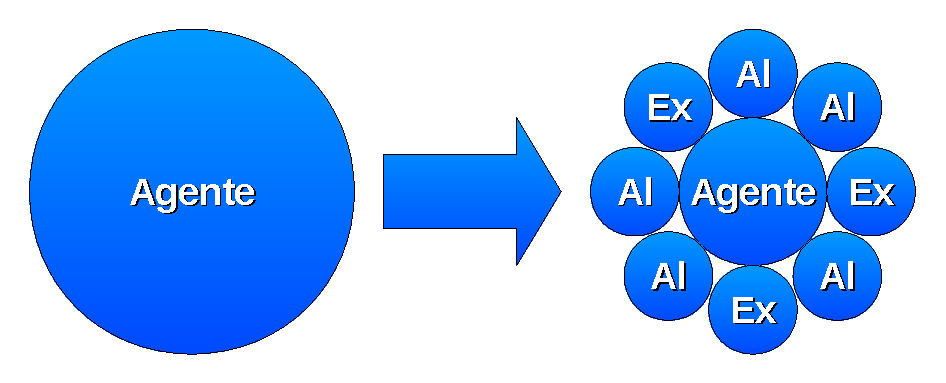
\includegraphics[width=0.7\textwidth]{images/nuevo_agente.pdf}
		\end{figure}

	\end{center}
\end{frame}

\subsection{Nuevo controlador}
\begin{frame}{Nuevo controlador}
	Se ha rehecho el controlador tratando de:
	\pause
	\begin{itemize}
		\item Mejorar la interfaz
		\item Mejorar el rendimiento
		\begin{itemize}
			\item Disminuir los accesos a base de datos
			\item Reducir los tiempos de operación
			\item Delegando en el navegador
		\end{itemize}
	\end{itemize}
\end{frame}

\begin{frame}{Nuevo controlador}
	\begin{center}
		Se ha hecho uso del \emph{framework} MVC CakePHP que simplifica enormemente el desarrollo.
	\end{center}
\end{frame}

\begin{frame}{Nuevo controlador}
	\only<1>{
		\begin{figure}
			%\centering
			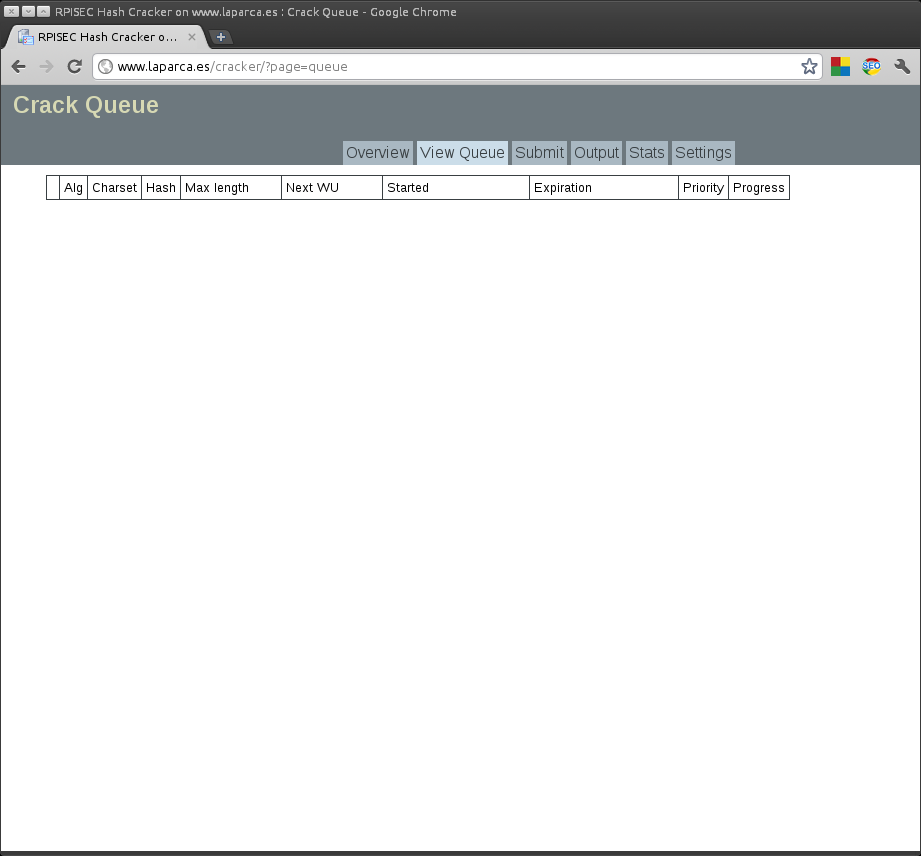
\includegraphics[width=0.7\textwidth]{images/cola_vieja.png}
		\end{figure}
	}
	\only<2>{
		\begin{figure}
			%\centering
			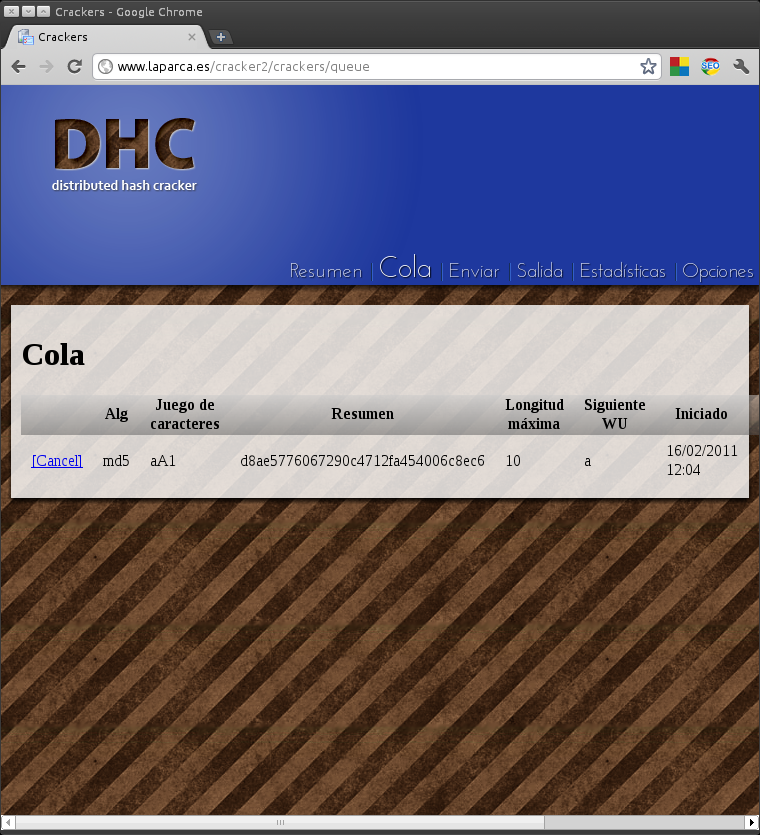
\includegraphics[width=0.6\textwidth]{images/cola.png}
		\end{figure}
	}
\end{frame}

\section{Presupuesto}
\mysection{Presupuesto}

\begin{frame}{Presupuesto}
	\begin{center}
		El precio final del proyecto es de \color{green}43.785,30\euro{} \color{white} y su duración ha sido de 11 meses, trabajado unas 13,2 horas semanales.
	\end{center}
\end{frame}

%\begin{frame}{Presupuesto}

%	Se han tenido en cuenta todos los gastos de un desarrollo real:
%	\pause
%	\begin{itemize}
%		\item Gastos directos
%		\begin{itemize}
%			\item Sueldos \color{green}9.200,00\euro
%			\item Subcontratas \color{green}186,89\euro
%			\item Equipos \color{green}9.610,00\euro
%		\end{itemize}
%		\item Gastos indirectos \color{green}7.918,63\euro
%		\item Amortizaciones \color{green}70,80\euro
%		\item Colchón de riesgos \color{green}10\%
%		\item Beneficio \color{green}25\%
%	\end{itemize}
%\end{frame}

%\begin{frame}{Presupuesto}
%	\begin{center}
%		Precio final del proyecto contando el 18\% de I.V.A.
%		\pause
%		\only<2>{\Huge 43.785,30\euro}
%	\end{center}
%\end{frame}


\section{Conclusiones y trabajos futuros}
\mysection{Conclusiones y trabajos futuros}

\subsection{Conclusiones}
\begin{frame}{Conclusiones}
	\begin{itemize}
		\item Se ha conseguido mejorar la mantenibilidad de la solución
		\item Gracias a los plugins es más fácil ampliar DHC
		\item Usar \emph{frameworks} MVC facilita el desarrollo web
		\item El nuevo diseño del controlador lo hace más atractivo
	\end{itemize}
\end{frame}

\begin{frame}{Conclusiones}
	\begin{center}
		Gracias a todos estos cambios es más sencillo usar la tarjeta gráfica y comprobar contraseñas.
	\end{center}
\end{frame}

\begin{frame}{Conclusiones}
	\begin{center}
		Hay que tener muy en cuenta la calidad de las contraseñas para evitar intrusiones no deseadas.
	\end{center}
\end{frame}

\subsection{Trabajos futuros}
\begin{frame}{Trabajos futuros}
	\begin{itemize}
		\item Mejorar el protocolo de comunicaciones
		\item Centralizar los plugins en el controlador
		\item Más algoritmos y \emph{executors}
		\item Nuevos protocolos de seguridad
		\item Jerarquías y distribución de controladores
	\end{itemize}
\end{frame}

\begin{frame}
	\begin{center}
		\Huge Fin
	\end{center}
\end{frame}

%\section{Bibliografía}
%\begin{frame}[allowframebreaks]{Bibliografía}
%	\bibliographystyle{alpha}
%	\bibliography{bibliografia}
%\end{frame}
\end{document}
